\underbar{\textbf{\large Ejercicio 1:}} Suponga que hay que desarrollar la interfaz de usuario de una aplicación. Dicha interfaz estará formada por menús, opciones y formularios.\\ Hay que tener en cuenta que:

\begin{itemize}
  \item Desde cada menú se puede ejecutar una serie de opciones.
  \item La selección de una opción desencadena la activación de un formulario.
  \item Una opción solo puede aparecer en un menú, pero un mismo formulario puede ser compartido por varias opciones.
\end{itemize}

\begin{figure}[h]
  \begin{center}
    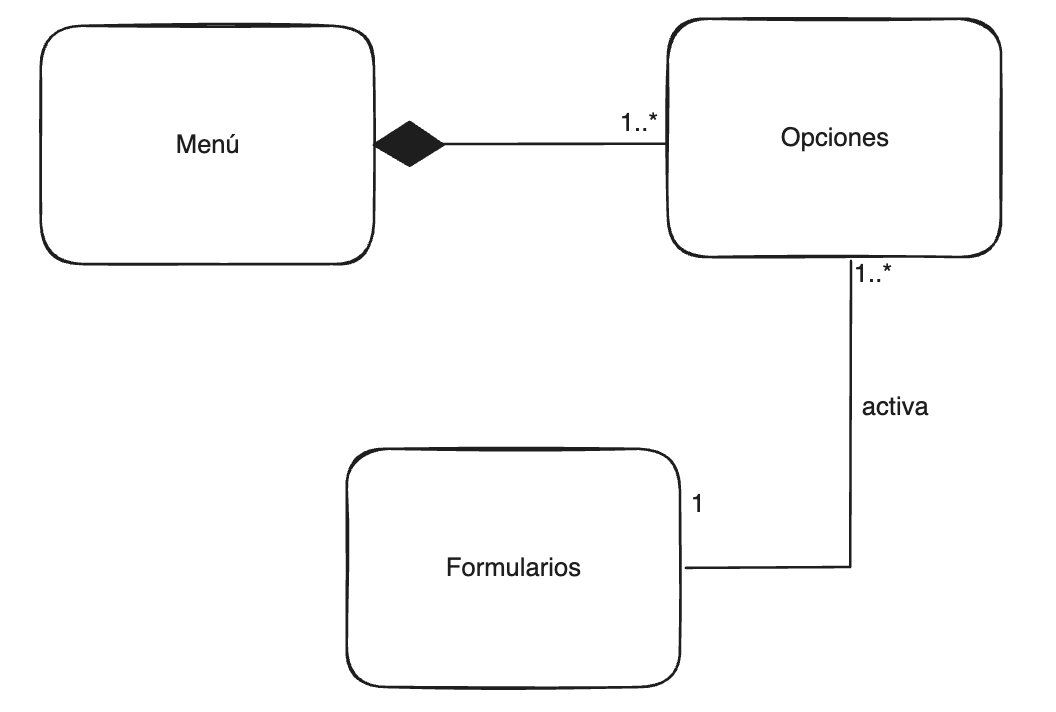
\includegraphics[width=\textwidth]{assets/Seminario3_1_1.png}
  \end{center}  
  \caption{Solución diagrama de clases }
\end{figure}

Implementación de las clases del diagrama de clases:
\begin{minted}[breaklines]{C++}
  class Menu{
    public: 
      typedef std::set<Opciones>ConjuntoOpciones;
      Menu(Opciones& opcion){}
      void setOpciones(Opciones* o)noexcept;
      friend bool operator < (const Menu& , const Menu& )noexcept;
    private:
      ConjuntoOpciones opciones_;
  };

  class Opciones{
    public:
      Opciones(Formularios& f):formulario_(&f){}
    private:
      Formularios* formulario_;
  };

  class Fomularios{
    public:
      typedef std::set<Opciones*>COpciones;
      Fomularios(Opciones& opcion){
        setOpciones(opcion);
      }
      void setOpciones(Opciones& o){
        opciones_.insert(&o);
      }
      const COpciones& getOpciones()const noexcept{return opciones_;}
    private:
      COpciones opciones_;
  };

  
\end{minted}
\underbar{\textbf{\large Ejercicio 2:}} Implemente las clases del diagrama, declarando exclusivamente los miembros imprescindibles para implementar las relaciones.

\begin{figure}[h]
  \begin{center}
    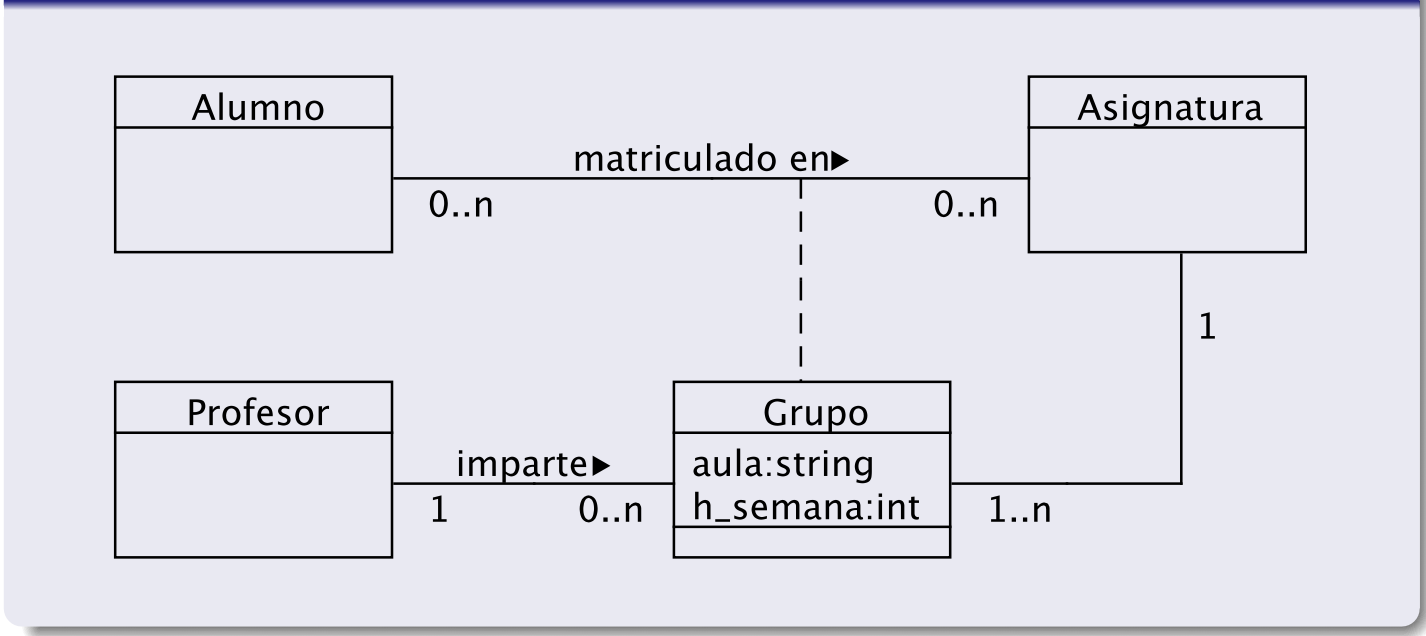
\includegraphics[width=\textwidth]{assets/Seminario3_1_2.png}
  \end{center}
\end{figure}

\begin{minted}[breaklines]{C++}
  class Alumno{
    public:
      //Alias del diccionario Asignatura - Grupo
      typedef std::map<Asignatura*,Grupo*>Asignaturas;
      void matriculados_en(Asignatura&, Grupo& )noexcept;
      const Asignaturas& getAsignaturas()const noexcept;
    private:
      Asignaturas asignaturas_;
  };
  class Asignatura{
    public:
      //Alias del diccionario Alumno - Grupo
      typedef std::map<Alumno*,Grupo*>Alumnos;
      void matricula(Alumno& , Grupo&)noexcept;
      const Alumnos& getAlumnos()const noexcept;
      //Alias del conjunto de Grupos de cada Asignatura
      typedef std::set<Grupo*>Grupos;
      void setGrupo(Grupo& )noexcept;
      const Grupos& getGrupo()const noexcept;
    private:
      Alumnos alumnos_;
      Grupos grupos_;
  };
  class Profesor; //Declaración adelantada
  class Grupo{
    public:
      Grupo(std::string a, int h, Asignatura& asig,Profesor& p): aula(a),h_semana(h),asignatura_(&asig),profesor_(&p){}
    private:  
      std::string aula;
      int h_semana;
      Asignatura* asignatura_;
      Profesor* profesor_;
  };
  class Profesor{
    public:
      //Alias del conjunto de Grupos de un profesor
      typedef std::set<Grupo*>Grupos;
      void imparte(Grupo&)noexcept;
      const Grupos& getGrupos()const noexcept;
    private:
      Grupos grupos;
  };

\end{minted}

\underbar{\textbf{\large Ejercicio 3:}} Defina los dos métodos siguientes:

\begin{itemize}
  \item \textbf{Alumno::matriculado\_en()} para matricular a un alumno en una asignatura asignándole un grupo.
\begin{minted}[breaklines]{C++}
void Alumno::matriculados_en(Asignatura& asig, Grupo& g)noexcept{
  asignaturas_.insert(std::make_pair(&asig,&g));
}
\end{minted}
  \item \textbf{Profesor::imparte()} para vincular un profesor a un grupo.
\begin{minted}[breaklines]{C++}
void Profesor::imparte(Grupo& g)noexcept{
  grupos_.insert(&g);
}
\end{minted}
\end{itemize}
\newpage
\underbar{\textbf{\large Ejercicio 4:}} Declare una clase de asociación Alumno\_Asignatura para la relación matriculado\_en. Para ello declare los atributos que considere necesarios, dos métodos \texttt{matriculado\_en()} y \texttt{matriculados()}. El primero registra a un alumno en una asignatura asignándole el grupo y el segundo devuelve todas las asignaturas (y los correspondientes grupos) en que se encuentre matriculado un alumno. Declare sobrecargas de estos dos métodos para el otro sentido de la asociación.
\begin{minted}[breaklines]{C++}
  class Alumno_Asignatura{
    public:
      //Alias de los diccionarios de Alumno y Asignatura con Grupos
      typedef std::map<Alumno*,Grupo*> Alumnos;
      typedef std::map<Asignatura*,Grupo*>Asignaturas;
      //Alias de los diccionarios de la relacion
      typedef std::map<Alumno*,Asignaturas> Alum_Asig;
      typedef std::map<Asignatura*,Alumnos>Asig_Alum;
      //Relaciona las clases
      void matriculados_en(Alumno&, Asignatura&, Grupo&)noexcept;
      void matriculados_en(Asignatura&, Alumno&, Grupo&)noexcept;
      //observadores de la clase
      Alumnos matriculados(Asignatura& )const noexcept;
      Asignaturas matriculados(Alumno& )const noexcept;
    private:
      Alum_Asig directa_;
      Asig_Alum inversa_;
  };



\end{minted}

\underbar{\textbf{\large Ejercicio 5:} }Declare una clase de asociación Profesor\_Grupo para la relación imparte. Incluya en ella los atributos oportunos y dos métodos \texttt{imparte()} e \texttt{impartidos()}. El primero enlaza un profesor con un grupo y el segundo devuelve todos los grupos que imparte un profesor. Sobrecargue ambas funciones miembro para el sentido inverso de la relación.
\begin{minted}[breaklines]{C++}
  class Profesor_Grupo{
    public:
      //Alias de los diccionarios de la relacion
      typedef std::set<Grupo*>Grupos;
      typedef std::map<Profesor*,Grupos>Profe_Grupo;
      typedef std::map<Grupo*,Profesor*>Grupo_Profe;
      //relaciona las clases
      void imparte(Profesor&, Grupo&)noexcept;
      void imparte(Grupo&,Profesor&)noexcept;
      //Observadores de la clase
      Grupos impartidos(Profesor& )const noexcept;
      const Profesor* impartidos(Grupo& )const noexcept;
    private:
      Profe_Grupo directa_;
      Grupo_Profe inversa_;
  };
\end{minted}
\newpage
\underbar{\textbf{\large Ejercicio 6:}} Defina el método \textbf{alumno\_Asignatura::matriculado\_en()} (y su sobrecarga) para matricular a un alumno en una asignatura asignándole un grupo. Esta función también permitirá cambiar el grupo al que pertenece un alumno ya matriculado en la  asignatura.
\begin{minted}[breaklines]{C++}
  void Alumno_Asignatura::matriculados_en(Alumno &alumno, Asignatura& asig, Grupo& grupo)noexcept{
    directa_[&alumno].insert(std::make_pair(&asig,&grupo));
    inversa_[&asig].insert(std::make_pair(&alumno,&grupo));
  }
  void Alumno_Asignatura::matriculados_en(Asignatura& asig, Alumno& alumno, Grupo& grupo)noexcept{
  matriculados_en(alumno,asig,grupo); //delegamos en el método anterior.
}
\end{minted}
\underbar{\textbf{\large Ejercicio 7:}} Escriba la definición de \textbf{Profesor\_Grupo::imparte()}. Si el grupo ya tiene un profesor asociado, se deberá desvincular del mismo y enlazarlo con el nuevo.
\begin{minted}[breaklines]{C++}
  void Profesor_Grupo::imparte(Profesor& prof, Grupo& grupo)noexcept{
    directa_[&prof].insert(&grupo);
    inversa_[&grupo]=&prof;
  }
  void Profesor_Grupo::imparte(Grupo& grupo, Profesor& prof)noexcept{
    imparte(prof,grupo);
  }
\end{minted}
\underbar{\textbf{\large Ejercicio 8:}} Defina \textbf{Profesor\_Grupo::impartidos()}.
\begin{minted}[breaklines]{C++}
  Profesor_Grupo::Grupos Profesor_Grupo::impartidos(Profesor& p)const noexcept{
    //Buscamos si el profesor está relacionado
    auto i = directa_.find(&p);
    if(i!=directa_.end()) return i->second;
    else{
      Profesor_Grupo::Grupos vacio;
      return vacio;
      //return std::set<Grupo*>();
    }
  }

  const Profesor* Profesor_Grupo::impartidos(Grupo& g)const noexcept{
    auto i = inversa_.find(&g);
    if(i!=inversa_.end()) return i->second;
    else{
      return nullptr;
    }
  }
\end{minted}
